\section{Performance Evaluation}
\label{sec:snarkprobe-evaluation}

Our first set of evaluations for \tool explores its performance and scalability.
All experiments run on an Intel Core i7-8700 CPU @ 3.20\,GHz $\times$ 12 with 32\,GB of RAM running 64-bit Ubuntu 22.04 LTS.

\subsection{Performance of the \ConstraintChecker}
We start by testing the \ConstraintChecker and evaluate its performance on statements with different types of operations and complexities, and present the runtimes in Table \ref{tab:snarkprobe-performance1}.
There are two runtime results for each experiment.  We first recorded the runtime for the SMT solver, which is the most important step in the \ConstraintChecker, and we also recorded the total runtime, including the processing time of the Circuit Extractor, SMT solver, and other internal evaluations.

We tested different types of proofs, including the well-known cube example, a comparison (which requires using a gadget), a hash (a complicated mathematics equation), and a proof with inner product, logical operators, and comparison (which requires multiple gadgets and more complex logic). As expected, as we progress in terms of ``complexity'', runtime generally increases.  Interestingly, the hash proof takes the longest in the SMT solver, demonstrating that there are different notions of ``complexity'' than just statement size.

%\clg{We observed that processing time is generally determined by the specific relations in circuit, which depends on the runtime to solve the equations by SMT solver. Interestingly, a large, ``complicated'' R1CS matrix or statement equation may not need a longer time to be evaluated by the \ConstraintChecker, since the ``complicated'' R1CS matrix may actually be easy for the SMT solver to handle.} \clg{Maybe remove this text since we don't have any way to back it up or justify it?} 

We also sought to test if the correctness of the statement checked had any impact on performance.  We did this by running two different experiments with the cube proof, one where we model a developer correctly flattening the statement equation into R1CS, and a second where we model a mistake in the flattening that introduces an error. Our \ConstraintChecker took a shorter time to evaluate the incorrect cube program since the \ConstraintChecker aborts as soon as it finds an error (such as a different domain or output value). 

\begin{table}[t]
\centering
\begin{adjustbox}{max width=\textwidth}
\begin{tabular}{c|c|cc}
\hline
\multirow{2}{*}{Statement} & \multirow{2}{*}{Equation} & \multicolumn{2}{c}{Runtime (in seconds)} \\ \cline{3-4} 
                           &                           & \multicolumn{1}{c|}{SMT Solver}     & Overall    \\ \hline\hline
Cube                       & $y = x^3 + x + 5$         & \multicolumn{1}{c|}{0.49}           & 4.18       \\ \hline
Cube with Error            & $y = x^3 + x + 5$         & \multicolumn{1}{c|}{0.24}           & 3.94       \\ \hline
Comparison                 & $x < 60$                  & \multicolumn{1}{c|}{0.54}           & 12.39      \\ \hline
SHA-256 Hash               & $y = \texttt{sha256}(x)$    & \multicolumn{1}{c|}{0.71}           & 15.39      \\ \hline
Inner Product        & $\langle u,v \rangle < c_1 \land \langle u,v \rangle > c_2$ & \multicolumn{1}{c|}{0.59}           & 18.34      \\ \hline
\end{tabular}
\end{adjustbox}
\caption{\ConstraintChecker runtime for different proof statements}
\label{tab:snarkprobe-performance1}
\vspace*{-20pt}
\end{table}

%%%%%%%%%

\subsection{Performance of \SnarkFuzzer}
\label{subsec:snarkprobe-performance-fuzzer}

We tested \SnarkFuzzer on \libsnark, \bellman, \arkworks, and \gnark to evaluate the processing time and performance in different configurations.
All experiments run on a single core, except for the \valuemonitor which is trivially parallelizable across all cores.
We start by evaluating the overall tool to examine the runtime percentage that is dedicated to each sub-component.  We then drill down and individually explore the scalability of each sub-component to gain a fuller understanding of \SnarkFuzzer's overall scalability. % We discuss the most influential performance results here, and provide additional benchmarks in Appendix~\ref{app:additionalgraphs}.

%%%%%

\parhead{Overall Runtime with Different Libraries and Protocols.}
We first explore the proportion of total running time that each different facet of \SnarkFuzzer takes, and present the results in Figure~\ref{fig:snarkprobe-time}.

We ran with five different configurations: \libsnark with \pinocchio, \libsnark with \groth16, \bellman with \groth16, \arkworks with \groth16, and \gnark with \groth16. All of these experiments use generation-based fuzzers to produce valid R1CS matrices (the slowest of the four fuzzing methods we provide) with dimensions in $[30,60]$.  We ran 30 iterations of the \branchmodel (since as shown in Figure~\ref{fig:snarkprobe-coverage} that provides reasonable coverage) and calculated the average runtime to complete a full ``run''\footnote{We define a ``full run'' to be using the \inputgenerator to produce one zkSNARK program, analyzing coverage status with the \branchmodel, and looking for any software and cryptographic related bugs with the \valuemodel and \valuemonitor.} and proof check for each library and protocol.

\begin{figure}[t]
  \centering
  %\captionsetup{justification=centering}
  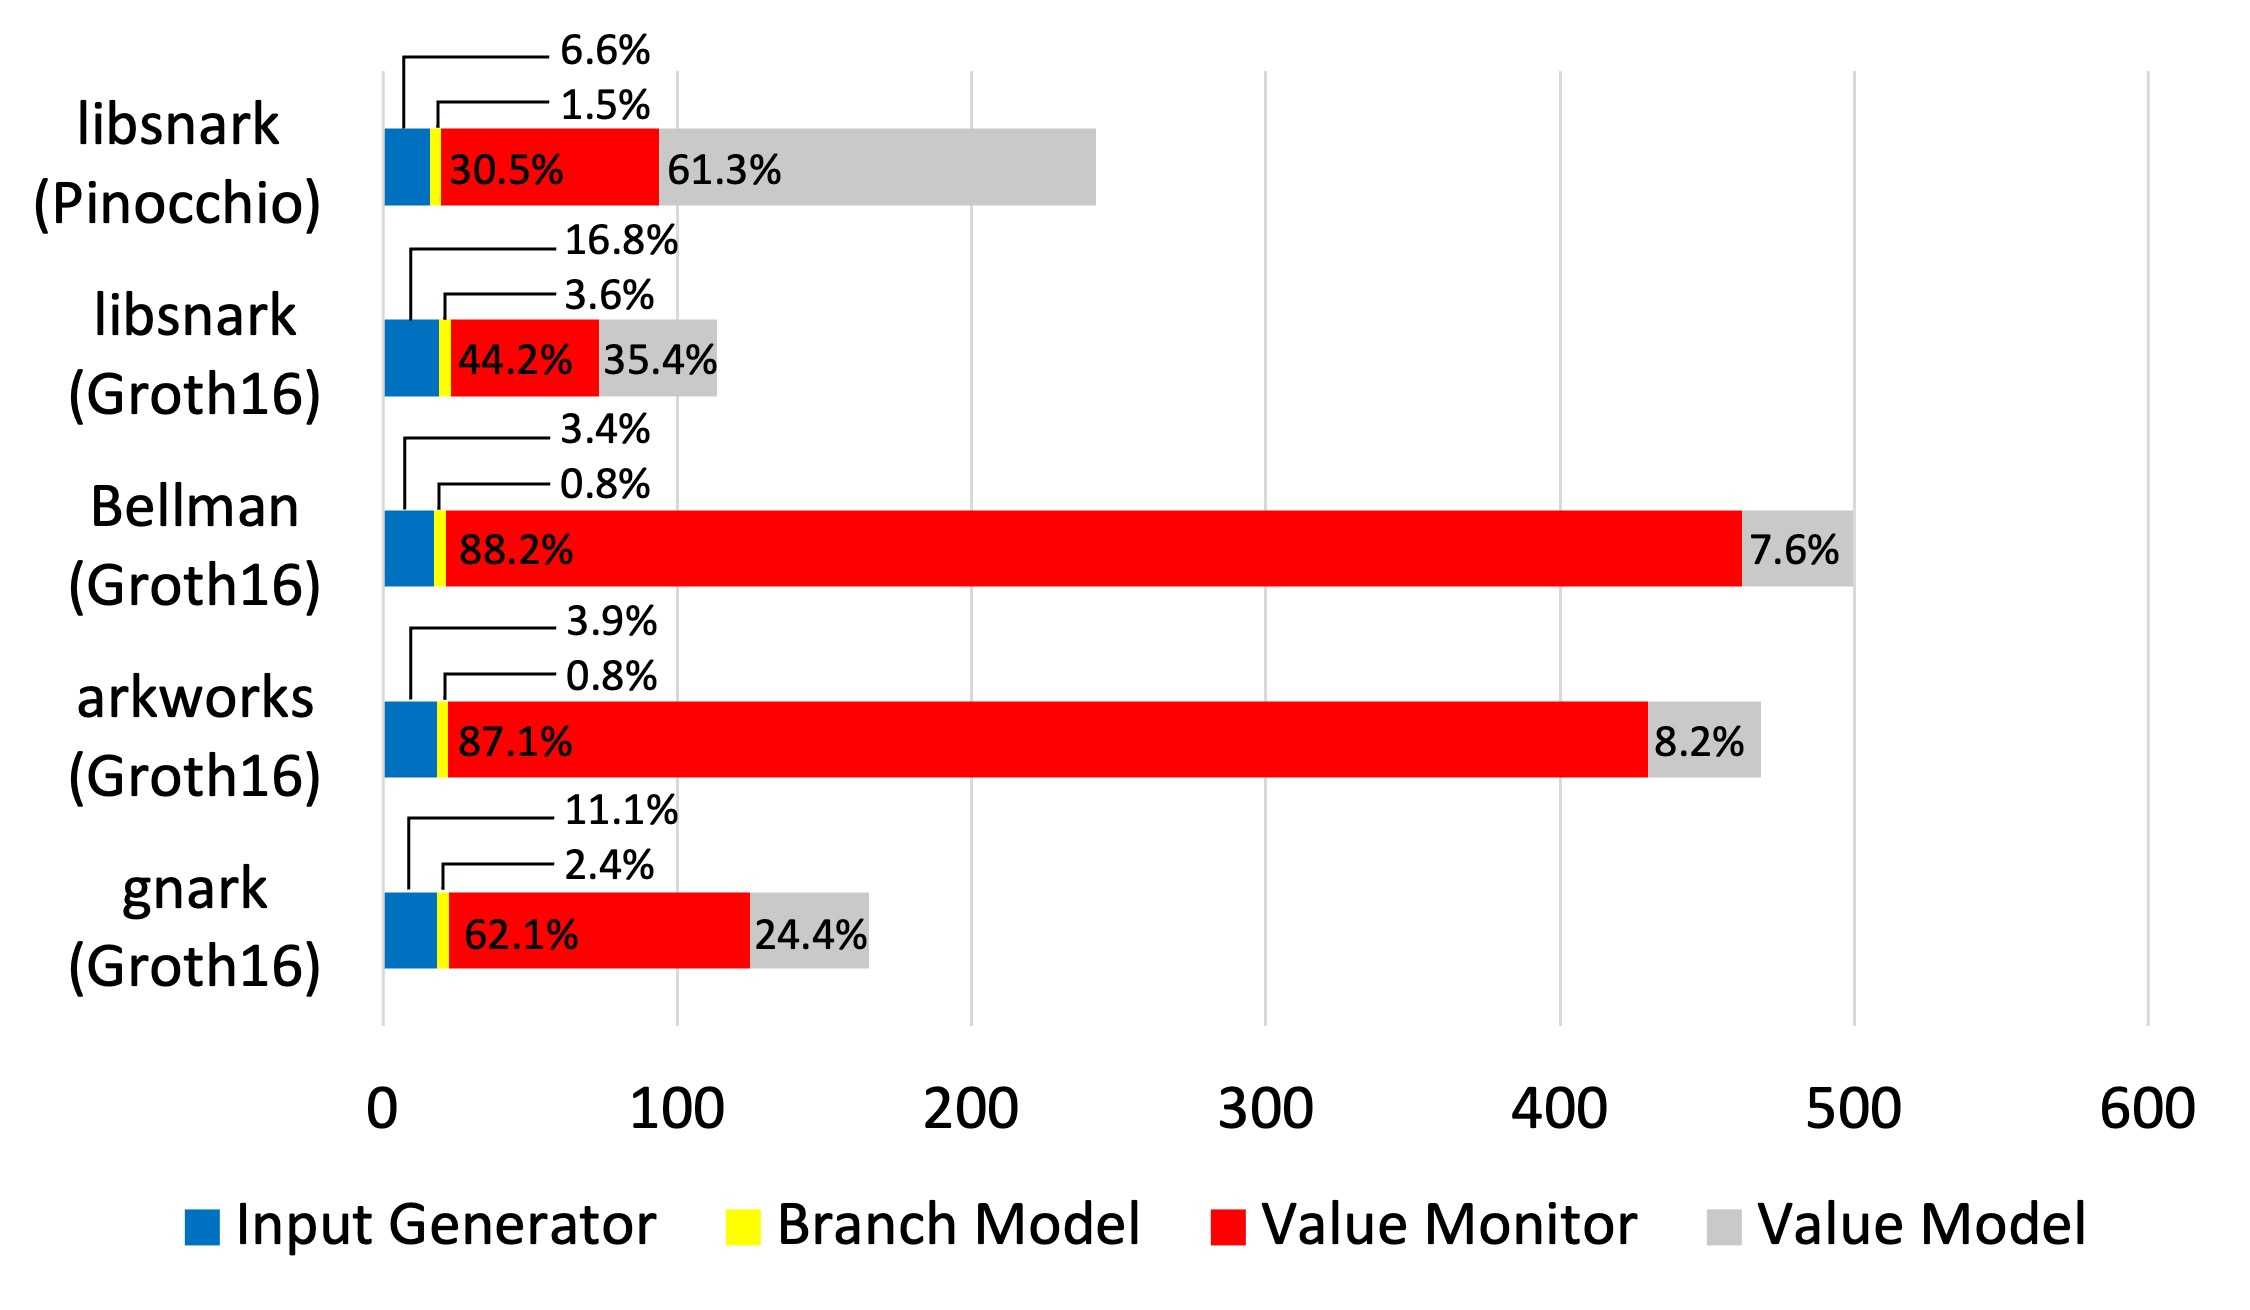
\includegraphics[width=0.8\linewidth]{ch-snarkprobe/figure/time.jpg}
	\vspace*{-10pt}
  \caption{Runtime of each component in \SnarkFuzzer with different libraries and protocols, both in terms of actual time as well as percentage of the total.}
  \label{fig:snarkprobe-time}
\vspace*{-10pt}
\end{figure}

%As we can see, the overall runtime is reasonable even in this slowest configuration, taking roughly 280 seconds for \libsnark with \pinocchio, 130 seconds for \libsnark with \groth16, and 580 seconds for \bellman with \groth16 to complete a full ``run''\footnote{We define a ``full run'' to be using the \inputgenerator to produce one zkSNARK program, analyzing coverage status with the \branchmodel, and looking for any software and cryptographic related bugs with the \valuemodel and \valuemonitor.} and proof check.

We observe that for all libraries and protocols, the majority of time is spent in the \valuemonitor and \valuemodel phases.  This is somewhat expected, as the cryptographic operations in the \valuemodel require time to calculate, and Valgrind's simulation hardware watch also introduces substantial overhead.  Since \groth16 has fewer elliptic curve and pairing operations than \pinocchio, testing that involves \groth16 costs less time. However, Valgrind spends a longer time executing a program in Rust than a program in C and Go. Since we use Valgrind in the \valuemonitor to find and monitor value changes, we see a longer overall runtime with \bellman and \arkworks than \libsnark and \gnark.

We do use small R1CS matrices in these experiments, as the primary goal is to demonstrate the runtime proportion for each component.  We make a few key observations about this.  We noticed that unless one uses only generation-based fuzzing to produce valid inputs, the size of the R1CS matrix (i.e., the proof) will not substantially affect the performance of the \inputgenerator.  The \branchmodel does not work with the R1CS matrix, so different sizes will result in the same runtime.
However, a large matrix will significantly increase the runtime of the \valuemodel and \valuemonitor (see Table~\ref{tab:snarkprobe-performance2} for more realistic values).  For total runtime reference, an R1CS matrix of size $100 \times 5000$ takes about 940 seconds to run the complete \SnarkFuzzer with our generation-based invalid matrix fuzzer.

%As we discussed previously, we are enable to trivially enable parallel running for the \valuemonitor across multiple CPU cores to reduce its percentage of processing time.  This is because the \valuemonitor watches all variables defined in the ideal value file, and unlike the \valuemodel, watching a single variable does not require communication with any other variables that need to be watched.

%We note that there are a number of avenues for optimization that would decrease the overall runtime.
%Switching to a different mechanism for the \valuemonitor could also decrease performance as well, and we will discuss the performance improvement in Section \ref{subsubsec:scalability}.

%%%%%


\parhead{Performance of the \inputgenerator.}
Unlike a mutation-based or generation-based fuzzer for an invalid matrix (which are very quick since they only require straightforward operations), generating a valid R1CS matrix with our generation-based fuzzer requires the SMT solver to produce a matrix based on the random witness array. Thus the processing time depends on the matrix size and random value(s) in the witness list, which generally results in a larger matrix taking longer to process.
To validate this, we used our various fuzzers to produce matrices of varying sizes (remember that the rows represent the number of constraints and columns the number of variables). In Table \ref{tab:snarkprobe-gen-invalid}, we present the processing time for each method (generally under one second for most methods), which confirms our general intuition.
We also note that the \inputgenerator must compile the input matrix (proof) and source code into a binary program, which can require substantial time that is outside of our control.
%Some \zksnark libraries may require longer compiling time, and we have no control to the library compiling time cost, which will increase our \inputgenerator total runtime.
%\delete{ Although a larger matrix usually takes a longer time to generate, a ``smaller'' R1CS matrix may also require greater computational resources depending on the random numbers chosen in the witness and R1CS relations, as this can cause simplified relations in R1CS matrix and witness, thus requiring the SMT solver to take less time to calculate a valid R1CS matrix.\yuquan{Might need better explanation for this line?}  For example, we can see that matrix three and matrix seven in the 10 × 200 category only take roughly ten seconds to generate, which is similar to generating a matrix of size 20 × 40.} \fanyo{(summary)}

%\begin{figure}[t]
  %\centering
  %%\captionsetup{justification=centering}
  %\includegraphics[width=0.9\linewidth]{imgs/gen-invalid.jpg}
  %\caption{Runtime of the \inputgenerator to produce R1CS matrices of different sizes.}
  %\label{fig:snarkprobe-gen-invalid}
%\end{figure}

\begin{table}[h]
\centering
\begin{adjustbox}{max width=\textwidth}
\begin{tabular}{ll||c|c|c|c}
\hline
\multicolumn{2}{l||}{Matrix Size} & $5 \times 10$ & $20 \times 40$ & $50 \times 100$ & $50 \times 200$ \\ \hline\hline
\multicolumn{1}{l||}{\multirow{2}{*}{}Generation Based} & Invalid Matrix & \textless{}0.01 & \textless{}0.01 & \textless{}0.01 & 0.02 \\ \cline{2-6}
\multicolumn{1}{l||}{} & Valid Matrix & 0.16 & 2.06 & 23.02 & 51.27 \\ \hline
\multicolumn{1}{l||}{\multirow{2}{*}{}Mutation Based} & Invalid Matrix & 0.38 & 0.49 & 0.65 & 0.77 \\ \cline{2-6}
\multicolumn{1}{l||}{} & Valid Matrix & \textless{}0.01 & \textless{}0.01 & \textless{}0.01 & 0.02 \\ \hline
\end{tabular}
\end{adjustbox}
\caption{Runtime (in seconds) of the \inputgenerator to produce R1CS matrices of different sizes.}
\label{tab:snarkprobe-gen-invalid}
% \vspace*{-14pt}
\end{table}

%%%%

\parhead{Performance of the \branchmodel.}
Next, we explore the coverage ability of the \branchmodel in terms of breadth, as well as how quickly we achieve a high percentage of branch coverage.  We ran 50 iterations of the \branchmodel with \libsnark, which covers more than 85\% of all branches.  We stopped our experiments after 50 iterations as \SnarkFuzzer did not reach any new branches over the previous 10 prior iterations.  Even with this, we note that after roughly 30 iterations we see the breadth of our coverage begin to taper off.
A graph can be found in Figure \ref{fig:snarkprobe-coverage}.
%\fanyo{Even the \tool have covered most pf the branches in the target libraries, the fuzzer should not be stopped in order to generate more different inputs to test a same branch. The fuzzer should not be stopped until most of the branches have been tested for at least one time. As more inputs are generated, \tool has higher chance to find the potential issues in the target library or higher confidence to say (need a better word) that the target library is safe. }
%There are a number of factors that can affect our coverage results. First, we can encounter situations where the generation-based fuzzer cannot produce enough diverse input sets to cover all branches, which is where the seeds of the mutation-based fuzzer can play an important role in coverage.  Second, \SnarkFuzzer allows a user to configure the proportion of matrices generated by each sub-fuzzing method, which can also affect the coverage result. In our experiment, we had the generation-based fuzzer produce 5\% invalid and 45\% valid matrices, and the mutation-based fuzzer produce 40\% invalid and 10\% valid matrices. Increasing the fuzzing time and/or adding extra seeds for the mutation-based fuzzer can improve the coverage of a target source library.

\begin{figure}[h]
  \centering
  %\captionsetup{justification=centering}
  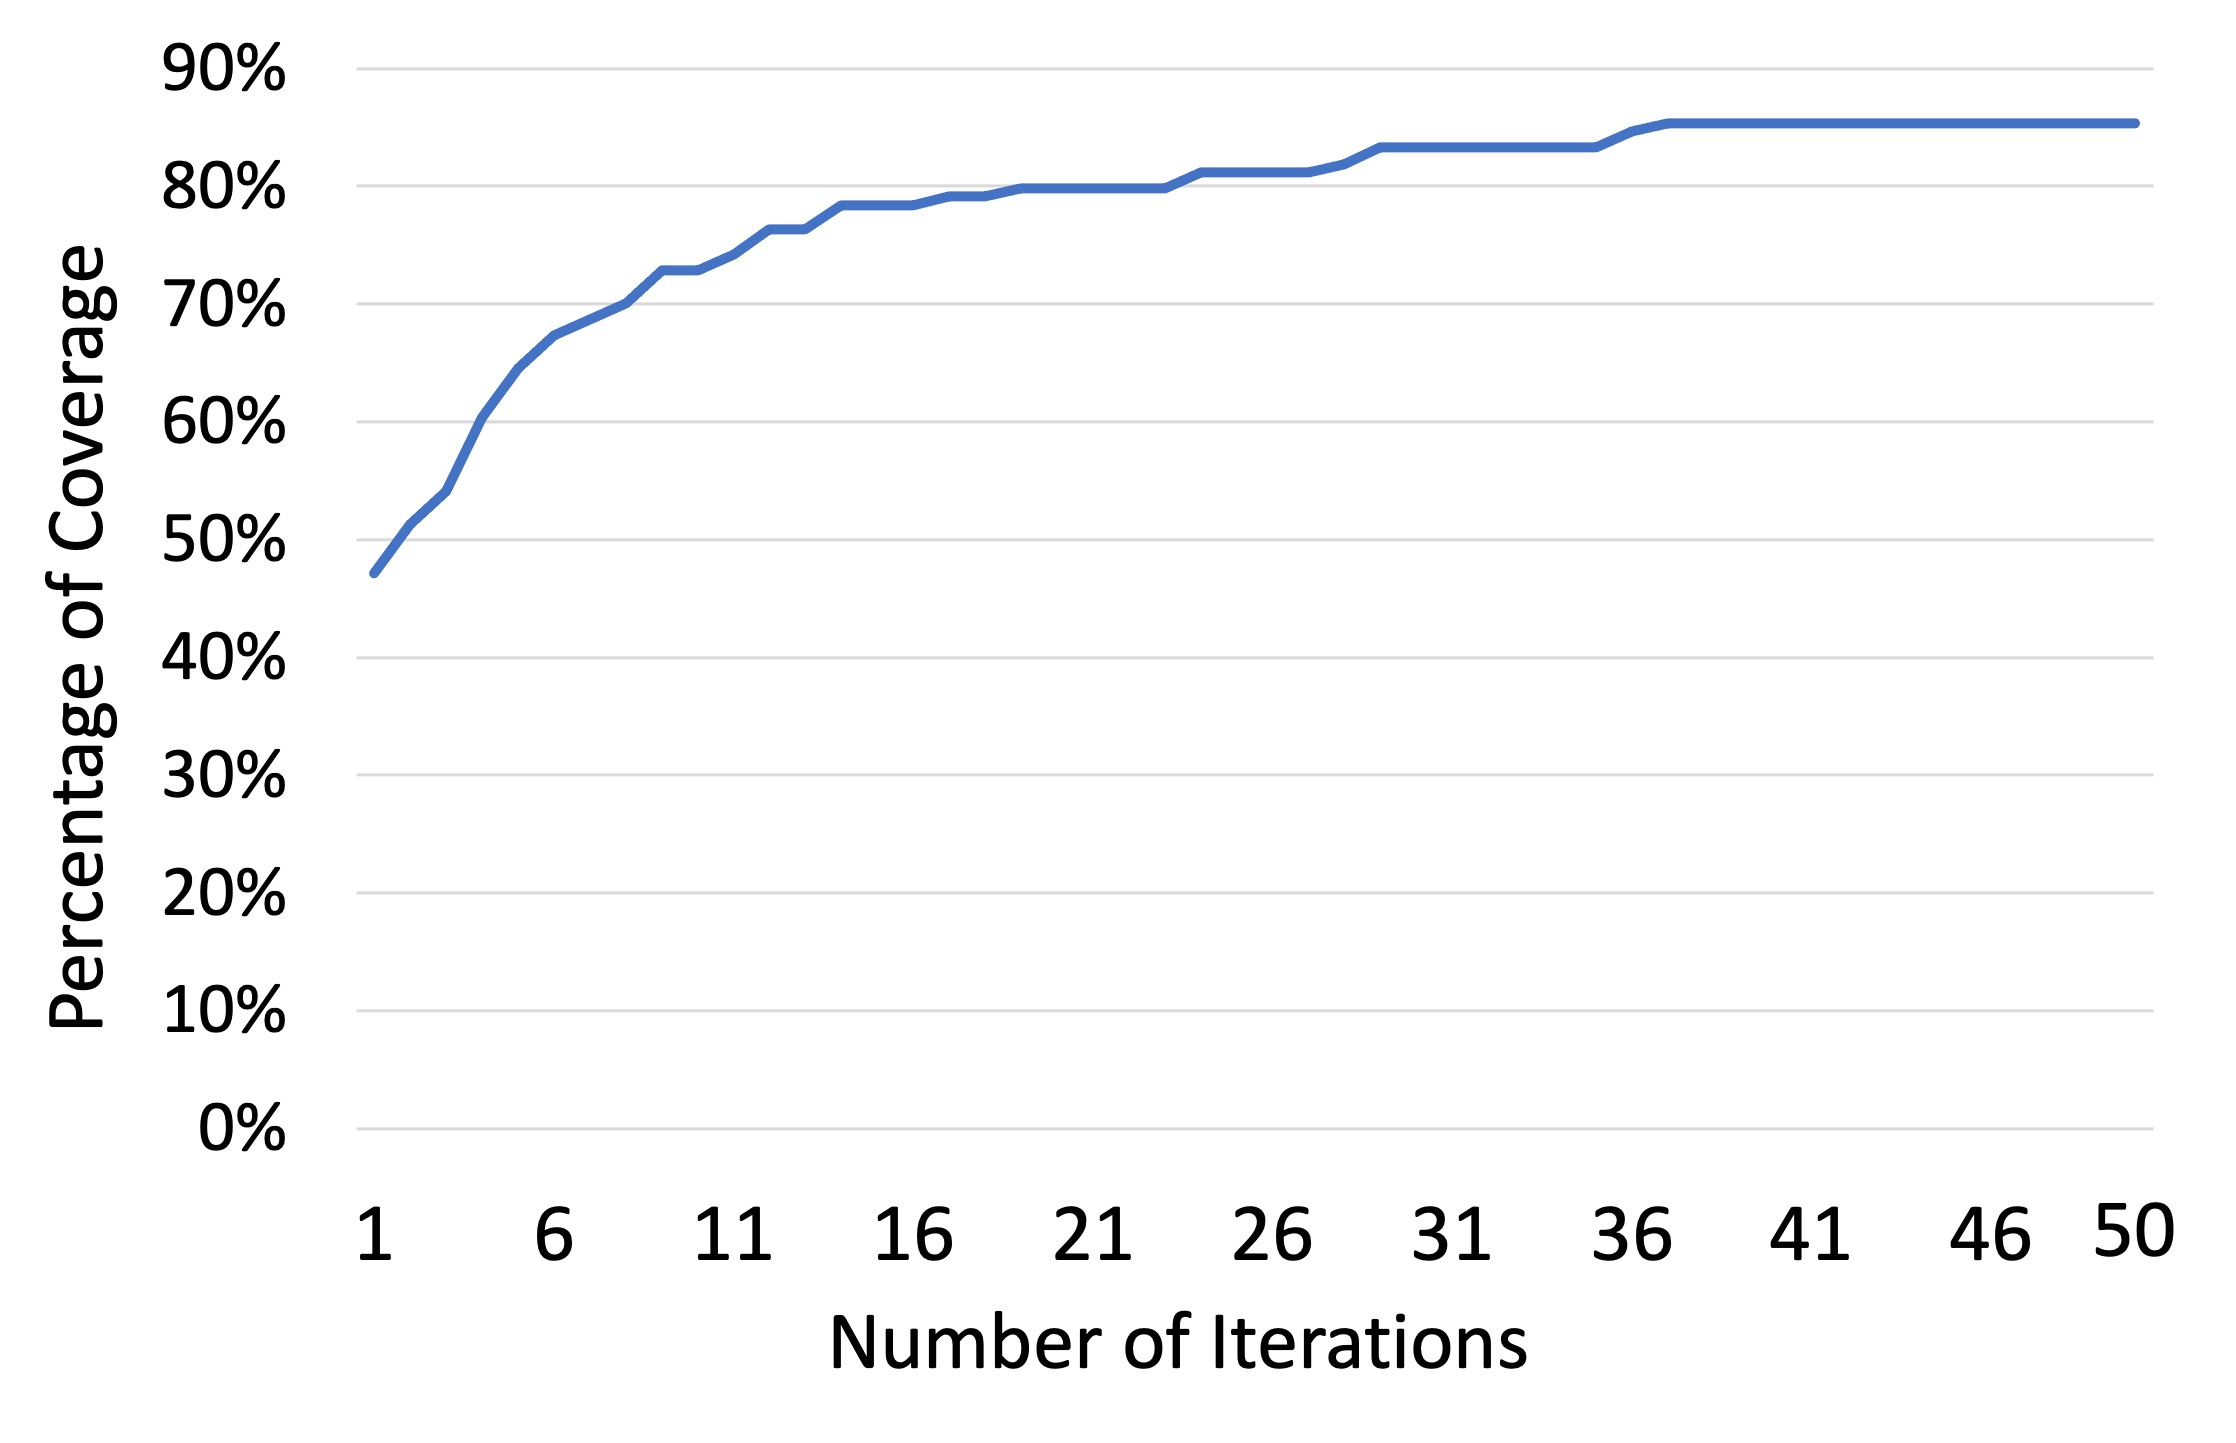
\includegraphics[width=0.70\linewidth]{ch-snarkprobe/figure/coverage.jpg}
  \vspace*{-10pt}
  \caption{Percentage (breadth) of library coverage after a given number of iterations}
  \label{fig:snarkprobe-coverage}
  %\vspace*{-8pt}
\end{figure}

%%%%%%%%%%


\parhead{Performance of \valuemodel and \valuemonitor.}
The primary effects on overall performance are our \valuemodel and \valuemonitor.  Table \ref{tab:snarkprobe-performance2} shows the runtime with different matrix sizes.  We expect the size of our matrices to be one of the primary influences on the runtime of these components.

Recall that the computation of the proving key requires calculations with the circuit.
%, such as \[ pk_A := \{A_{i}(\tau)\alpha_{A}\rho_{A}\mathcal{P}\}_{i=0}^{m+3} \] in \pinocchio protocol \cite{ben2014succinct} and \[ v(x) = \sum_{k=0}^{m} a_{k} v_{k} (x) \] in \groth16 protocol \cite{nitulescu2020zk}.
Therefore, a larger R1CS matrix will result in longer runtime in our \valuemodel. At the same time, the shape of the matrix will also affect its runtime. As we can see in Table \ref{tab:snarkprobe-performance2}, a matrix of size $20 \times 45$ takes less time than one of size $30 \times 30$ or $45 \times 20$, even though they all contain 900 integers. In fact, the number of variables (columns) plays a greater role than the number of constraints (rows) in \valuemodel runtime, since this plays a larger role in the size of the proving and verification keys. %For example, a matrix of size 45 × 20 has fewer integers than a matrix of size 45 × 60, but the \valuemodel spends similar runtime (around 41 seconds) to re-evaluate the programs with these two matrices. \yuquan{If we are showing that number of columns has greater influnece on runtime than number of rows, I think a comparison between 20 × 45 (29.52s) and 60 × 45 (46.03s) makes more sense? Maybe just add "In contrast, the Value Model runtime difference between 20 × 45 matrix and 60 × 45 matrix reaches 16.51 seconds."}

Similarly, the \valuemonitor requires more time to watch variables in a program with a larger matrix. However, the reason for this is different.  Since the runtime of Valgrind depends on the space complexity of a variable, the matrix shape will not have an effect. Instead, the \valuemonitor spends more time monitoring a program with a larger matrix, but it takes similar time for programs with the same number of integers but different shapes.  For example, each matrix of size $20 \times 45$, $30 \times 30$, and $45 \times 20$ has 900 integers, and the \valuemonitor takes around 46 seconds to run, even though they have a different shape.

\begin{table}[t]
\centering
\begin{adjustbox}{max width=\textwidth}
\begin{tabular}{cc||cc}
\hline
\multicolumn{2}{c||}{Matrix Setting} & \multicolumn{2}{c}{Processing Time (in second)} \\ \hline
\multicolumn{1}{c|}{Matrix Size} & Items in Matrix & \multicolumn{1}{c|}{\valuemodel} & \valuemonitor \\ \hline\hline
\multicolumn{1}{c|}{$10 \times 30$} & 100 & \multicolumn{1}{c|}{23.33} & 29.21 \\ \hline
\multicolumn{1}{c|}{$10 \times 30$} & \multirow{2}{*}{300} & \multicolumn{1}{c|}{25.96} & 33.09 \\ \cline{1-1} \cline{3-4} 
\multicolumn{1}{c|}{$30 \times 10$} &  & \multicolumn{1}{c|}{32.78} & 34.21 \\ \hline
\multicolumn{1}{c|}{$20 \times 45$} & \multirow{3}{*}{900} & \multicolumn{1}{c|}{29.52} & 43.99 \\ \cline{1-1} \cline{3-4} 
\multicolumn{1}{c|}{$30 \times 30$} &  & \multicolumn{1}{c|}{33.01} & 46.30 \\ \cline{1-1} \cline{3-4} 
\multicolumn{1}{c|}{$45 \times 20$} &  & \multicolumn{1}{c|}{40.14} & 47.68 \\ \hline
\multicolumn{1}{c|}{$45 \times 60$} & \multirow{2}{*}{2700} & \multicolumn{1}{c|}{41.29} & 81.69 \\ \cline{1-1} \cline{3-4} 
\multicolumn{1}{c|}{$60 \times 45$} &  & \multicolumn{1}{c|}{46.03} & 80.21 \\ \hline
\multicolumn{1}{c|}{$100 \times 1500$} & 150000 & \multicolumn{1}{c|}{200.84} & 223.49 \\ \hline
\multicolumn{1}{c|}{$100 \times 5000$} & 500000 & \multicolumn{1}{c|}{580.97} & 344.83 \\ \hline
\end{tabular}
\end{adjustbox}
\caption{Runtime of the \valuemodel and \valuemonitor to process an R1CS matrix of varying size.  For example, $10 \times 30$ is a matrix with 10 variables and 30 constraints.}
\label{tab:snarkprobe-performance2}
% \vspace*{-14pt}
\end{table}

\parhead{Discussion of Total Runtime.}
Our experiments only provide an upper bound on the worst case runtime for \SnarkFuzzer.  We did not perform any runtime optimizations, and in all of our experiments, we used the slowest options or configurations that we knew of.
While \SnarkFuzzer does require extra runtime in the \valuemonitor and \valuechecker for each individual input seed, in comparison to a traditional fuzzer, which might spend hundreds or thousands of core hours to produce inputs, the \framework and \branchmodel designs allow\SnarkFuzzer to find issues with a relatively small number of generated input seeds.
In fact, most errors that \SnarkFuzzer detected (see Section \ref{sec:snarkprobe-errorcatching}) were found with less than ten seeds.
Therefore, we view performance to be acceptable for real world usage.

%%%%%

\iffalse

\subsection{Scalability and Paths to Improvement}
\label{subsec:snarkprobe-scalability}

Finally, we conclude our performance evaluation with a brief discussion about the scalability of \SnarkFuzzer.
Our experiments only provide an upper bound on the worst case runtime for \SnarkFuzzer.  We did not enable or perform any runtime optimizations (except for parallel running in the \valuemonitor).  And in all of our experiments, we used the slowest options or configurations that we knew of (for example, we computed the overall tool runtime in Figure~\ref{fig:time} using the slowest of our fuzzing options).  We tested on a wide variety of R1CS matrix sizes and configurations, which are representative of statements of varying complexity (recall that the number of constraints in R1CS roughly maps to the number of gates in an arithmetic circuit).  In all of these instances, we view performance to be acceptable for real world usage, as nothing takes more than tens of minutes to run overall.

%we used z3py (a Z3 API in Python) to generate a valid R1CS matrix in the \inputgenerator because it was easy to use and integrated with our framework \clg{Why did we pick this one and not, say Z3, which is popular, again?}. Comparing with standard Z3 or other high performance theorem provers, z3py is especially slow at solving an equation with many variables.
However, there are several paths to reduce the processing time further.
For example, the \inputgenerator could be sped up by replacing z3py with another theorem prover in a lower level language or by new SMT solvers \cite{Parafrost-OsamaWB-tacas21, fpsmtgpu, osama2021gpu} that can be accelerated by a GPU.
For the \valuemonitor and \valuemodel, we note that our implementation choices can (easily) be replaced by other similar techniques to improve runtime. For example, when testing a library that does not contain any large data structures, GDB hardware watch might be the right choice to monitor variables instead of Valgrind, as this is extremely efficient (but can only watch a limited number of variables at a time). And the \valuechecker could be enhanced by parallelization, though one must be careful to handle core communication since some values must be calculated in a specific order.

\fi

%\begin{table}[h]
%\centering
%\begin{tabular}{|l|l|l|l|}
%\hline
%Library            & \multicolumn{2}{l|}{\libsnark} & \bellman \\ \hline
%Protocol           & PGHR13 & Groth16 & Groth16 \\ \hline
%Total Variables    & 78     & 44      &         \\ \hline
%Integer            & 6      & 1       &         \\ \hline
%Finite Field       & 12     & 6       &         \\ \hline
%G1                 & 20     & 13      &         \\ \hline
%G2                 & 14     & 11      &         \\ \hline
%Finite Field Array & 8      & 4       &         \\ \hline
%G1 Array           & 17     &         &         \\ \hline
%G2 Array           & 1      &         &         \\ \hline
%
%\end{tabular}
%\caption{Extractor}
%\label{tab:extractor}
%\end{table}

%%%%%%%%%%
